\documentclass[]{article}
\usepackage{lmodern}
\usepackage{amssymb,amsmath}
\usepackage{ifxetex,ifluatex}
\usepackage{fixltx2e} % provides \textsubscript
\ifnum 0\ifxetex 1\fi\ifluatex 1\fi=0 % if pdftex
  \usepackage[T1]{fontenc}
  \usepackage[utf8]{inputenc}
\else % if luatex or xelatex
  \ifxetex
    \usepackage{mathspec}
  \else
    \usepackage{fontspec}
  \fi
  \defaultfontfeatures{Ligatures=TeX,Scale=MatchLowercase}
\fi
% use upquote if available, for straight quotes in verbatim environments
\IfFileExists{upquote.sty}{\usepackage{upquote}}{}
% use microtype if available
\IfFileExists{microtype.sty}{%
\usepackage{microtype}
\UseMicrotypeSet[protrusion]{basicmath} % disable protrusion for tt fonts
}{}
\usepackage[margin=1in]{geometry}
\usepackage{hyperref}
\hypersetup{unicode=true,
            pdftitle={Proiect},
            pdfborder={0 0 0},
            breaklinks=true}
\urlstyle{same}  % don't use monospace font for urls
\usepackage{graphicx,grffile}
\makeatletter
\def\maxwidth{\ifdim\Gin@nat@width>\linewidth\linewidth\else\Gin@nat@width\fi}
\def\maxheight{\ifdim\Gin@nat@height>\textheight\textheight\else\Gin@nat@height\fi}
\makeatother
% Scale images if necessary, so that they will not overflow the page
% margins by default, and it is still possible to overwrite the defaults
% using explicit options in \includegraphics[width, height, ...]{}
\setkeys{Gin}{width=\maxwidth,height=\maxheight,keepaspectratio}
\IfFileExists{parskip.sty}{%
\usepackage{parskip}
}{% else
\setlength{\parindent}{0pt}
\setlength{\parskip}{6pt plus 2pt minus 1pt}
}
\setlength{\emergencystretch}{3em}  % prevent overfull lines
\providecommand{\tightlist}{%
  \setlength{\itemsep}{0pt}\setlength{\parskip}{0pt}}
\setcounter{secnumdepth}{0}
% Redefines (sub)paragraphs to behave more like sections
\ifx\paragraph\undefined\else
\let\oldparagraph\paragraph
\renewcommand{\paragraph}[1]{\oldparagraph{#1}\mbox{}}
\fi
\ifx\subparagraph\undefined\else
\let\oldsubparagraph\subparagraph
\renewcommand{\subparagraph}[1]{\oldsubparagraph{#1}\mbox{}}
\fi

%%% Use protect on footnotes to avoid problems with footnotes in titles
\let\rmarkdownfootnote\footnote%
\def\footnote{\protect\rmarkdownfootnote}

%%% Change title format to be more compact
\usepackage{titling}

% Create subtitle command for use in maketitle
\newcommand{\subtitle}[1]{
  \posttitle{
    \begin{center}\large#1\end{center}
    }
}

\setlength{\droptitle}{-2em}
  \title{Proiect}
  \pretitle{\vspace{\droptitle}\centering\huge}
  \posttitle{\par}
  \author{}
  \preauthor{}\postauthor{}
  \date{}
  \predate{}\postdate{}

%%%%%%%%%%%%%%%%%%%%%%%%%%%%%%%%%%%%%%%%%%%%%%%%%%%%%%%%%%%%%%%%%%%%%%%%%%%%%%%%%%%%%%%%%%%%%%%%%%%%%%%%%%%%%%%%%%%%%
\usepackage{subfigure}
\usepackage{booktabs}
\usepackage{slashbox}
\usepackage{color}
\usepackage{caption}
\usepackage{graphicx}
%%%%%%%%%%%%%%%%%%%%%%%%%%%%%%%%%%%%%%%%%%%%%%%%%%%%%%%%%%%%%%%%%%%%%%%%%%%%%%%%%%%%%%%%%%%%%%%%%%%%%%%%%%%%%%%%%%%%%
%CITEVA DEFINITII
\def\om{\omega}
\def\Om{\Omega}
\def\et{\eta}
\def\td{\tilde{\delta}}
\def\m{{\mu}}
\def\n{{\nu}}
\def\k{{\kappa}}
\def\l{{\lambda}}
\def\L{{\Lambda}}
\def\g{{\gamma}}
\def\a{{\alpha}}
\def\e{{\varepsilon}}
\def\b{{\beta}}
\def\G{{\Gamma}}
\def\d{{\delta}}
\def\D{{\Delta}}
\def\T{{\Theta}}
\def\t{{\theta}}
\def\s{{\sigma}}
\def\S{{\Sigma}}
\def\z{{\zeta}}
\def\qed{\hfill\Box}
\def\ds{\displaystyle}
\def\mc{\mathcal}
%%%%%%%%%%%%%%%%%%%%%%%%%%%%%%%%%%%%%%%%%%%%%%%%%%%%%%%%%%%%%%%%%%%%%%%%%%%%%%%%%%%%%%%%%%%%%%%%%%%%%%%%%%%%%%%%%%%%%%
\def\1{{\mathbf 1}}
\def\CC{{\mathbb C}}
\def\RR{{\mathbb R}}
\def\QQ{{\mathbb Q}}
\def\ZZ{{\mathbb Z}}
\def\PP{{\mathbb P}}
\def\EE{{\mathbb E}}
\def\VV{{\mathbb V}}
\def\NN{{\mathbb N}}
\def\FF{{\mathbb F}}
%\def\SS{{\mathbb S}}
\def\MO{{\mathcal O}}
\def\MA{{\mathcal A}}
\def\MF{{\mathcal F}}
\def\MR{{\mathcal R}}
\def\MB{{\mathcal B}}
\def\MM{{\mathcal M}}
\def\MN{{\mathcal N}}
\def\MU{{\mathcal U}}
\def\MP{{\mathcal P}}
\def\MS{{\mathcal S}}
\def\MBS{{\mathbf S}}
\def\MX{{\bm{ \mathscr X}}}

% independent sign
\newcommand\independent{\protect\mathpalette{\protect\independenT}{\perp}}
\def\independenT#1#2{\mathrel{\rlap{$#1#2$}\mkern2mu{#1#2}}}

%%%%%%%%%%%%%%%%%%%%%%%%%%%%%%%%%%%%%%%%%%%%%%%%%%%%%%%%%%%%%%%%%%%%%%%%%%%%%%%%%%%%%%%%%%%%%%%%%%%%%%%%%%%%%%%%%%%%%
%Header and Footer
\usepackage{fancyhdr}

\pagestyle{fancy}
\fancyhf{}
\rhead{Universitatea din Bucure\c sti\\ Facultatea de Matematic\u a \c si Informatic\u a}
\lhead{\textit{Curs}: Biostatistic\u a 2016-2017\\ \textit{Instructor}: A. Am\u arioarei}
\rfoot{Pagina \thepage}
\lfoot{Grupa: 503}
%%%%%%%%%%%%%%%%%%%%%%%%%%%%%%%%%%%%%%%
\captionsetup[figure]{labelfont={bf},labelformat={default},name={Figura}} 
\captionsetup[table]{labelfont={bf},labelformat={default},name={Tabelul}}

\begin{document}
\maketitle

%%%%%%%%%%%%%%%%%%%%%%%%
\thispagestyle{fancy}

\subsubsection[Problema 1]{\texorpdfstring{Problema 1\footnote{Raportul
  poate fi scris in \emph{Word} sau \LaTeX (pentru u\c surin\c t\u a
  recomand folosirea pachetului \emph{rmarkdown} din \emph{R} - mai
  multe informa\c tii g\u asi\c ti pe site la sec\c tiune \emph{Link-uri
  utile}). Toate simul\u arile, figurile \c si codurile folosite trebuie
  incluse in raport. Se va folosi doar limbajul \emph{R}.}}{Problema 1}}\label{problema-1}

Populațiile diverselor specii de
\href{https://en.wikipedia.org/wiki/Drosophila_melanogaster}{\emph{Drosophila
melanogaster}} (musculița de vin/oțet sau a fructelor) prezintă variații
ale formei aripilor. Forma aripilor este cuantificată prin măsurarea
locațiilor unde nervurile se intersectează între ele sau se
intersectează cu marginile acestora (vezi Figura 1). Se obține un total
de 15 astfel de puncte de intersecție, fiecare având două coordonate,
prin urmare forma aripii este caracterizată de un vector din
\(\RR^{30}\).

\begin{figure}[htbp]
\centering
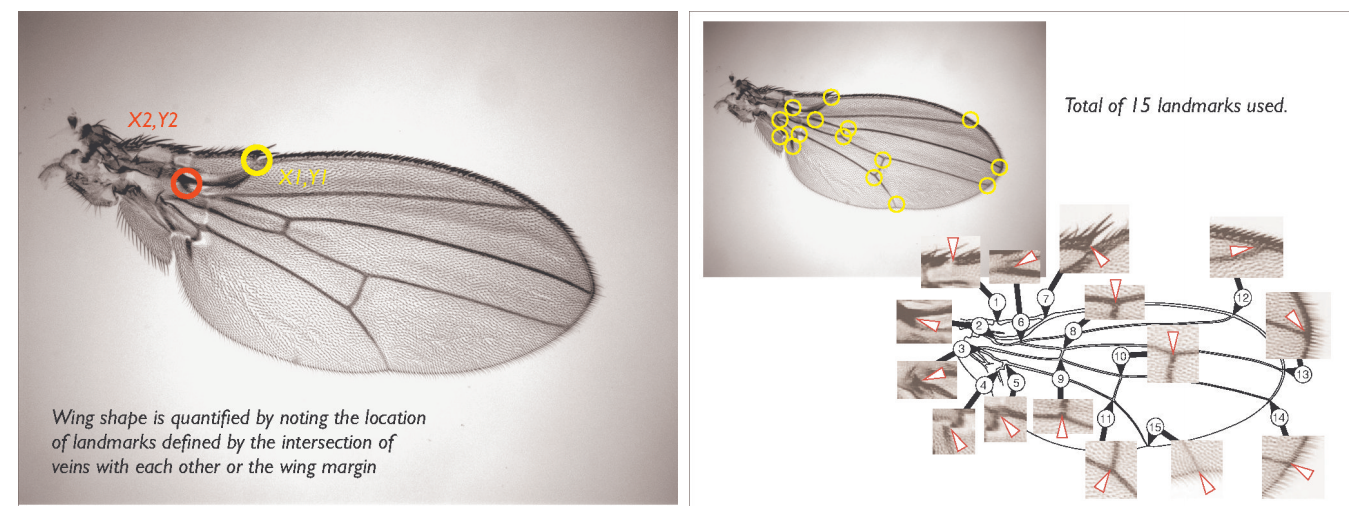
\includegraphics{Figs/Wing.png}
\caption{Cunatificarea formei unei aripi}
\end{figure}

Ne propunem să investigăm dacă forma aripilor poate diferenția
următoarele trei specii de musculițe: \emph{D. Mauritiana}, \emph{D.
Sechellia} și \emph{D. Simulans}. Pentru aceasta considerăm setul de
date \href{Data/wing.dat}{\texttt{wing.dat}} care conține cuantificarea
formei aripilor a 138 de musculițe de oțet diferite, fiecare făcând
parte dintr-una din cele 3 specii enumerate mai sus astfel: de la 1 la
42 din specia \emph{D. Mauritiana}, de la 43 la 90 din specia \emph{D.
Sechellia} iar restul din specia \emph{D. Simulans}. Fie \(\bf{Y}\)
matricea observațiilor și \(\bf{X}\) matricea \emph{centrată} obținută
prin \[
\bf{X}_{i,j} = \bf{Y}_{i,j}-\bar{\bf{Y}}_{\cdot, j}
\]

\begin{enumerate}
\def\labelenumi{\arabic{enumi}.}
\item
  Calculați matricea \(\bf{C}=\frac{1}{137}\bf{X}^\intercal\bf{X}\). Ce
  reprezintă această matrice ?
\item
  Calculați \(\l_{max}\) și \(\bf{v}_{max}\) cea mai mare valoare
  proprie a matricii \(\bf{C}\) și vectorul propriu corespunzător
  (folosiți funcția \texttt{eigen}).
\item
  Pentru fiecare musculiță \(i\), calculați proiecția pe direcția
  \(\bf{v}_{max}\) a vectorului centrat \(X_i\) (linia \(i\) din
  matricea \(\bf{X}\)) care cuantifică forma aripii acesteia,
  \(l_i = <X_i, \bf{v}_{max}>\). Acest scalar va fi folosit ca un
  cuantificator al formei aripii pentru musculița \(i\).
\item
  Verificați grafic și printr-un test adecvat dacă descriptorii \(l_i\)
  sunt repartizați normal pentru fiecare din cele trei specii în parte.
\item
  Folosiți un test adecvat pentru a verifica dacă mediile
  \(\mu_{Mauritiana}\) și \(\mu_{Sechellia}\) sunt egale, unde
  \(\mu_{Mauritiana}\) reprezintă media descriptorilor \(l_i\) pentru
  specia Mauritiana și respectiv \(\mu_{Sechellia}\) este media lui
  \(l_i\) pentru specia Sechellia. Repetați procedura și pentru
  celelalte două perechi.
\item
  Verificați dacă cele trei medii sunt egale între ele.
\end{enumerate}

Să presupunem că vrem să studiem efectul raportului dintre mărimea
aripii pe mărimea corpului pentru musculița de oțet și abilitatea
acesteia de a scăpa de un păianjen. Testăm ipoteza că musculițele cu un
corp mai greu relativ la mărimea aripilor sunt mai vulnerabile. Mai
multe musculițe cu un raport scăzut între mărimea aripilor și a corpului
(clasificate ca și \emph{ușoare}) au fost închise într-o cutie împreună
cu 2 păianjeni pentru o perioadă de 8 zile. Un experiment similar a avut
loc pentru musculițe cu un raport ridicat (clasificate ca \emph{grele}).
Numărul de musculițe care au fost consumate de păianjeni este prezentat
în Tabelul 1:

\begin{table}[ht]
\caption {numarul de musculite consumate}
  \begin{center}

    \begin{tabular}{c|c|c|c}
        & Usoare & Grele & Total\\
        \hline
      $\leq$ 48h & 16 & 27 & 43\\
      48-96h & 6 & 10 & 16 \\
      96-144h & 7 & 6 & 13 \\
      144-192h 5 & 7 & 12 \\
      \hline
      Supravietuit dupa 192h & 71 & 55 & 126\\
      \hline
      Total & 105 & 105 & 210
    \end{tabular}
  \end{center}
\end{table}

\begin{enumerate}
\def\labelenumi{\arabic{enumi}.}
\setcounter{enumi}{6}
\tightlist
\item
  Verificați dacă rata de incidență a consumului rămâne constantă de-a
  lungul timpului. Calculați p-valoarea prin trei teste diferite.
\end{enumerate}


\end{document}
